\documentclass[a4paper, 11pt]{article}
\usepackage{geometry}
\geometry{letterpaper, margin=1in}
\usepackage{graphicx}
\graphicspath{ {images/} }

\usepackage{amsmath}
\usepackage{amssymb}  
\usepackage{amsthm}
\usepackage{ulem}

\usepackage{enumitem}


\usepackage{pdfpages} % for including full pdf pages

% format to allow bolded theorems, corollaries, etc... 
\newtheorem*{theorem}{Theorem}
\newtheorem*{corollary}{Corollary}
\newtheorem*{lemma}{Lemma}
\newtheorem*{definition}{Definition}
\newtheorem*{Example}{Example} 
\newtheorem*{Remark}{Remark}

% stop typing \mathbb a thousand times 
\newcommand{\R}{\mathbb{R}}
\newcommand{\C}{\mathbb{C}}
\newcommand{\F}{\mathbb{F}}

% commands for bra-ket notation
\newcommand{\bra}[1]{\ensuremath{\left\langle#1\right|}}
\newcommand{\ket}[1]{\ensuremath{\left|#1\right\rangle}}
\newcommand{\bracket}[2]{\ensuremath{\left\langle #1 \middle| #2 \right\rangle}}
\newcommand{\matrixel}[3]{\ensuremath{\left\langle #1 \middle| #2 \middle| #3 \right\rangle}}
\newcommand{\expectation}[1]{\ensuremath{\left\langle #1 \right\rangle}}

% change margins for solution
\newenvironment{solution}{%
	\begin{list}{}{%
			\setlength{\topsep}{0pt}%
			\setlength{\leftmargin}{0.5cm}%
			\setlength{\rightmargin}{0.5cm}%
			\setlength{\listparindent}{\parindent}%
			\setlength{\itemindent}{\parindent}%
			\setlength{\parsep}{\parskip}%
		}%
		\item[]}{\end{list}}



\begin{document}
\noindent
\large\textbf{Homework 3} \hfill \textbf{John Waczak} \\
\normalsize MTH 434 \hfill  Date: \today \\
Dr. Tevian Dray \hfill worked w/ Ryan Tollefsen
\par\noindent\rule{\textwidth}{0.4pt} \\\\



\begin{enumerate}[leftmargin=0em]
\item \textbf{INTEGRATION ON THE SPHERE} Consider $\mathbb{S}^2$ which can be
  viewed as the surface in $\mathbb{E}^3$ satisfying $x^2+y^2+z^2=
  \text{constant}$. Equivalently, it is the two-dimensional surface with line
  element $ds^2 = r^2(d\theta^2+\sin^2\theta d\phi^2)$
  \begin{enumerate}[leftmargin=3em, label=(\alph*)]
  \item Let $\omega$ be the orientation on $\mathbb{S}^2$. Determine
    $\displaystyle\int_{\mathbb{S}^2}\omega$
    \begin{solution}
      We can rewrite the line element in the more suggestive form
      \begin{equation}
        ds^2 = r^2d\theta^2+r^2\sin^2\theta d\phi^2
      \end{equation}
      So that the orientation can be chosen as
      \begin{equation}
        \omega = rd\theta\wedge r\sin\theta d\phi
      \end{equation}
      Then integration of $\omega$ is as simple as dropping the wedges and
      making sure that the final answer has the correct sign. That is,
      \begin{align}
        \int_{\mathbb{S}^2}\omega &= \int_0^{2\pi}\int_0^\pi r^2\sin\theta d\theta d\phi \\
                                  &= r^2\int_0^{2\pi}\Big.(-\cos\theta)\Big|_0^\pi d\phi \\
                                  &= 2r^2\int_0^{2\pi}d\phi \\
                                  &= 4\pi r^2
      \end{align}
      which is precisely what we should expect for the area of the 2-sphere. 
    \end{solution}

  \item Let $\alpha\in\bigwedge^1(\mathbb{S}^2)$. Use Stoke's theorem to compute
    $\displaystyle\int_{\mathbb{S}^2}d\alpha$.
    \begin{solution}
      Recall that the sphere is a compact surface with no boundary (section
      16.7). Then stokes theorem gives
      \begin{align}
        \int_{\mathbb{S}^2}d\alpha &= \int_{\partial\mathbb{S}^2}\alpha \\
        &= \int_\varnothing\alpha = 0 
      \end{align}
      where in the last line we are integrating a 1-form over the empty set. 
    \end{solution}
    
  \item Find a 1-form on $\mathbb{S}^2$ such that $d\alpha = \omega$.
    \begin{solution}
      We can write a general 1-form as
      \begin{equation}
        \alpha = f\;rd\theta + h\;r\sin\theta d\phi
      \end{equation}
      Zapping with d gives (\textbf{Note:} $r$ is constant on $\mathbb{S}^2$)
      \begin{align}
        d\alpha &= r\left( \frac{\partial (h\sin\theta)}{\partial \theta} - \frac{\partial f}{\partial \phi} \right)d\theta\wedge d\phi \\
                &= \frac{1}{r\sin\theta}\left( \frac{\partial (h\sin\theta)}{\partial \theta} - \frac{\partial f}{\partial \phi} \right)rd\theta\wedge r\sin\theta d\phi \\
        \omega &= rd\theta \wedge r\sin\theta d\phi \\
        \Rightarrow r\sin\theta &= \left( \frac{\partial (h\sin\theta)}{\partial \theta} - \frac{\partial f}{\partial \phi} \right)
      \end{align}
      At this point we can make a choice. If we let $f=f(\theta)$ and
      $h=-r\cot(\theta)$, then we have
      \begin{align}
        r\sin\theta &= \frac{\partial(-r\cot\theta\sin\theta)}{\partial\theta} + 0 \\
        &= -r\frac{\partial\cos\theta}{\partial\theta} = r\sin\theta
      \end{align}
      Thus, if we let
      \begin{align}
        \alpha &= f(\theta)rd\theta-r^2\cos\theta d\phi
      \end{align}
    \end{solution}
  \item How is this possible?
    \begin{solution}
      As we can see, this appears to be a contradiction. In part (a) we found
      that integrating $\omega$ gives a non-zero value. Part (b) illustrated
      that $\omega$ can be written as an exterior derivative for which the
      integral over the whole $\mathbb{S}^2$ must be zero! How can we resolve
      this? If we allow our $f(\theta)=0$ then so far we have found that
      \begin{equation}
        \omega = d(-r^2\cos\theta d\phi)
      \end{equation}
      As the text says in section 20.4, ``the problem must be with $d\phi$''
      because $\cos\theta$ is certainly well defined over the whole circle.
      As the integral of $\omega$ is non-zero then $\omega$ must not be the
      derivative of a one form despite the fact that (17) is true. However, if
      (following the notation of section 20.4 of the text) we identify the
      orthonormal basis element as $r\sin\theta d\phi = \sigma^\phi$, then we may
      rewrite $\omega$ in terms of the orthonormal (well-behaved) basis element.
      \begin{equation}
        \omega = d(-r\cot\theta\sigma^\phi)
      \end{equation}
      In this form it is easy to see that because of the cotangent function,
      $\omega$ is undefined at the poles and therefore, $\omega$ itself
      is not a well-defined 2-form. This discrepancy must be what allows the integral
      to be non-zero. Certainly Stoke's theorem is correct but we also know that
      integrating the orientation over a surface should give the surface area.\\

      To aid in this consider the circle $\mathbb{S}^1$ for which $\omega =
      rd\theta$ If we integrate the orientation, we find that
      \begin{equation}
        \int_{\mathbb{S}^2}\omega = 2\pi r
      \end{equation}
      If we then apply stokes theorem to a one form, say $f=r\phi$ then we
      have $df = \omega$. Therefore, stokes theorem should give that the same
      integral (19) is 0. The resolution to the dilemma is that in order to apply
      Stoke's theorem, our integrand must be a smooth function over the whole
      region. This is \textit{not} the case for the coordinate function $\phi$
      because there is a sharp discontinuity between the angle $\phi=0$ and
      $\phi=2\pi$ which both correspond to the same position on the circle.\\

      On the 2-sphere, this issue persists so that, in fact, for half of the
      great circle between the north and south poles defined by $\phi=0$ there
      is a very \textit{not smooth} discontinuity in angle. This arc is shown in
      the following figure
      \begin{figure}[!hbt]
        \centering
        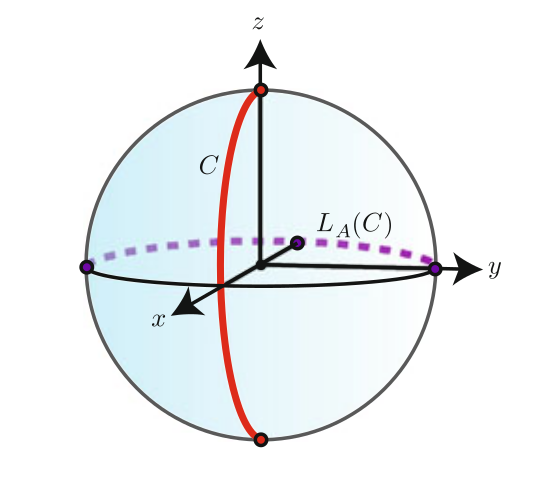
\includegraphics[width=0.65\columnwidth]{sphere_issue}
        \caption{Figure showing the sphere $\mathbb{S}^2$ with the half-great
          circle C illustrating the discontinuity in the angle $\phi$. Image
          taken from pg 131 of \textit{Differential Geometry of Curves and
            Surfaces} by K. Tapp.}
      \end{figure}

      Thus, the problem we faced was not really a problem at all but rather our choice
      of coordinates for the sphere does not satisfy the requirements for the
      application of stokes theorem to $\omega$. Our solution to part (b) is
      still correct because we never wrote the 1-form in terms of coordinates.
    
    \end{solution}
    
      
  \end{enumerate}
\end{enumerate}


\end{document}

































